\section{Research Plan} 
\label{sec:research}

% 35 pts for explanation here combined with timeline below

Re-state the problem you are trying to solve or question you are trying to
answer and then explain how you plan to solve/answer it. Is it evaluating a
visualization? Is it applying a human-centered technique from outside
visualization to your visualization design project? Is it running an
experiment to find out something about people? Is it synthesizing a large
body of literature? Is it something else?

Note this is a {\em plan}. The plan may change as you make discoveries during
your project. However, you must describe what your plan is assuming everything
goes as expected. If there are some parts of the plan where you could run into
difficulties, state what those difficulties are and what alternative measures
you could take should those difficulties arise.

You may refer to other sections so as not to repeat yourself -- for example,
referencing Section~\ref{sec:background}.

You may want to use figures to illustrate your point, such as
Figure~\ref{fig:sample}.

\begin{figure}[h]
 \centering % avoid the use of \begin{center}...\end{center} and use \centering instead (more compact)
 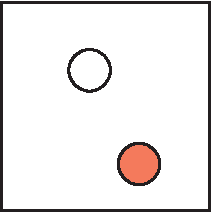
\includegraphics[width=1.5in]{figs/sample}
 \caption{Figure illustrating some proposed designs.}
 \label{fig:sample}
\end{figure}

% 10 pts
\subsection{Resources}
\label{sec:resources}

Describe any resources you need for this project here and whether or not you
already have access to them. If your project requires certain software, like
visualization systems to evaluate or survey software, do you have it? If not,
do you plan on writing it?

If your project needs data to visualization, describe whether you already have
access to the data and if not, what is required to obtain the data. If you
don't already have the data, explain how long it will take to retrieve it. 

If your project needs participants, how many do you foresee it needing, at
least for piloting? What kinds of skills must these people have? For example,
if you are working on a tool for analyzing octopi videos, does  it only make
sense to ask octopi experts?

The point of this section is to determine if you are prepared to do the
proposed work and if the milestones take into account these resources.

% 5 pts
\subsection{Technology}
\label{sec:tech}

Describe what if any technologies you intend to use (e.g., programming
languages, platforms, apps, existing libraries) and why they make sense for
your project. Do they serve your users better than other technologies? Are you
able to take advantage of existing work/libraries for your domain with this
technology rather than HTML/CSS/JS and d3js?  

\subsection{Timeline}
\label{sec:timeline}

Adapt the milestones for the class project to the specifics of your project
and summarize in Table~\ref{tab:milestones}. Do not simply copy the current
text as is. Your milestones should be specific to your problem.

The expectations are as follows:

\vspace{1.5ex}\noindent\textbf{Project Milestone Two} should include the
initial proposed methodology of any work you plan to do in detail, including
justification and rationale for why that methodology was chosen. It should
contain specifics of the design for your problem, such as how people will be
recruited, what they will be asked to do, and what artifacts need to be
generated, how the design is validated, and how results will be analyzed. Any
pre-studies/pilot work should also be in the plan.

If you are doing a literature review, you should have the methodology for how
you will find the literature and collect data based on it. For example, which
venues will you start with? What years? Keyword searches? What is your policy
for following citations?

No matter what kind of project you do, also compile an IRB proposal, including
all forms (e.g., F107), and consent documents. DO NOT submit it to the IRB, it
is for class use only. Do the proposal as if you were proposing Project
Milestone 2, unless you are doing a literature review. In that case, choose
one paper from your initial pool and fill out the IRB proposal as if you were
proposing that experiment.

Additionally, the related works should be updated with a more thorough
literature review. Changes to the status of the data and the choices of
technology should be discussed.

\vspace{1.5ex}\noindent\textbf{Project Milestone Three} should include
revisions following the project in-progress presentations as well as the
results of the first chunk of work that needs to be done. This first `chunk'
of work may involve implementation work (fixing interfaces, adding logging
features, creating visualizations for an experiment). Include images of these
implemented pieces and discussion of what they do. Demonstrations should run
with minimal effort and the code should be included in the repository.

Depending on needs, rather than coding, the chunk may involve piloting small
pieces of your design, decreasing factors in the study, or generating
experimental objects (e.g., more examples/trials/tutorials).

For projects involving heavy literature review, this milestone should include
annotations and notes for half of the selected papers.  Including a
preliminary schema for categorizing will help me give you feedback.

In the corresponding report, discussion of project progress as well as any
revisions to the data, methodology, technology choice, and scope should be
included.

\vspace{1.5ex}\noindent\textbf{Project Milestone Four} should include a
complete working prototype of the main project artifacts, such as the working
study with experimental objects and stimuli complete, the visualization tool
and evaluation script, or completed literature annotations with a
categorization scheme. The demonstration should run with minimal effort and
the code should be included in the repository.

If your project involves human participants directly, you should have also run
a pilot study by now with one or two volunteers. Report on the results of this
pilot---what worked? what didn't? what needs to be changed?

In the corresponding report, discussion of project progress as well as any
revisions to the data, technology choice, and scope should be included. The
plan for evaluation especially should be updated indicating the plan for
milestone five and any preliminary work in the design of that evaluation.


\vspace{1.5ex}\noindent\textbf{Project Milestone Five} should include the
final revisions of any study methodology, artifacts, or literature survey.
Additional pilots or study runs based on what was learned in the previous
milestone may be reported. If the study was run, analysis of the data
Artifacts generated (e.g., pre-observation plan, observation notes, data from
studies) during this study should be included in the repository.
Literature-based projects should include a refinement of the findings from the
previous milestone.

Additionally, this milestone should include reflection upon what was learned
in this project, with suggestions for people trying to do similar work.


\begin{table}[h]
%% Table captions on top in journal version
 \caption{Project Milestones}\vspace{1ex} % the \vspace adds some space after the top caption
 \label{tab:milestones}
 \scriptsize
 \centering % avoid the use of \begin{center}...\end{center} and use \centering instead (more compact)
   \begin{tabular}{r|r}
     Milestone & Description\\
   \hline
     PM2 & Choose methodology, put together initial study design, \\
	 & extend related work to include interaction studies in vis\\
     PM3 & Working version of interactive vis needed for study  \\
         & conditions, skeleton of code to advance questions. \\
     PM4 & Complete working version of study with consent and\\
         & tutorials, results of initial pilot with three people \\
     PM5 & Refinement off study based on pilot and pilot with three\\
         & new participants. Reflections on study design.\\
   \end{tabular}
\end{table}

